%! TEX root = icml_drau.tex
\section{Experiments}
\label{sec:exp}
%! TEX root = icml_drau.tex
\begin{figure*}[ht]
	\centering
	\includegraphics[width=\textwidth]{figs_data/full_results.pdf}
	\label{fig:full_results}
	\caption{Results on a variety of environments}
\end{figure*}

The experiments provided here are specifically aimed at showing that
the proposed method, DAU, works efficiently over a wide range of time
discretizations, without specific tuning, while standard deep $Q$-learning
approaches do not. DAU is compared to DDPG for continuous actions and to
DQN for
discrete actions.
Since we focus on $Q$-learning-like off-policy methods, we do not
compare against on-policy methods (A3C~\cite{a3c}, PPO~\cite{ppo},
TRPO~\cite{trpo}...).

In all setups, we use the algorithms described in
Alg.~\ref{alg:dau} and Supplementary Alg.~1. The variants of DDPG and DQN
used are described in the Supplementary, as well as all hyperparameters. We tested two different setups for DDPG and DQN.
In one, we scaled the discount factor (to avoid shortsightedness with small $\deltat$), but
left all other hyperparameters constant across time discretizations.
In the other, we used the properly rescaled discount
factor and reward from Eq.~\eqref{eq:def-gamma},
as well as $O(\deltat)$ learning rates for RMSProp.  The first variant yields slightly
better results, and is presented here, with the second variant in the
Supplementary.

Let us stress that the quantities plotted are rescaled to make comparison
possible across different timesteps. For example,
returns are given in terms of the discretized return $R_\deltat$ as defined in \eqref{eq:discretized-return},\footnote{This mostly amounts to scaling rewards
by a factor $\deltat$ when this scaling is not naturally done in the environment. Environment-specific
details are given in the Supplementary.} and, most notably, time elapsed is always given in
\emph{physical} time, i.e., the amount of time that the agent spent
interacting with the environment (this is not the number of steps).


\paragraph{Qualitative experiments: Visualizing policies and values.}
To provide qualitative results, and check robustness to time
discretization both in terms of returns and in terms
of convergence of the approximate value function and policies, we first provide results on the simple pendulum environment
from the OpenAI Gym classic control suite.  The state space is of
dimension $2$. We visualize both the learnt value and policy functions by
plotting, for each point of the phase diagram $(\theta, \dot{\theta})$,
its value and policy. The results are presented in
Fig.~\ref{fig:pend} (value function) and Figs.~1, 2,  3 in
Supplementary.

We plot the learnt policy at several instants in physical time
(normalized epochs) during training, for various time discretizations
$\deltat$, for both DAU and DDPG. With DAU, the agent's policy and value
function quickly converge for every time discretization without specific
tuning. On the contrary, with DDPG, learning of both value function and
policy vary greatly from one discretization to another.

\paragraph{Quantitative experiments.}
We benchmark DAU against DDPG on classic control benchmarks: Pendulum,
Cartpole, BipedalWalker, Ant, and Half-Cheetah environments from OpenAI Gym. On
Pendulum, Bipedal Walker and Ant, DAU is quite robust to variations of
$\deltat$ and displays reasonable performance in all cases. On the other hand,
DDPG's performance varies with $\deltat$; performance either degrades as
$\deltat$ decreases (Ant, Cheetah), or becomes more variable as learning
progresses (Pendulum) for small $\deltat$. On Cartpole, noise dominates,
making interpretation difficult. On Half-Cheetah, DAU is not clearly
invariant to time discretization. This could be explained by the multiple
suboptimal regimes that coexist in the Half-Cheetah environment (walking on the
head, walking on the back), which create discontinuities in the value
function (see Discussion).
% \begin{figure}[h]
%   \centering
%   \includegraphics[width=\columnwidth]{figs_data/cartpole_lc.png}
%   \caption{Cartpole}
%   \label{fig:cartpole-lc}
% \end{figure}

% \begin{figure}[h]
%   \centering
%   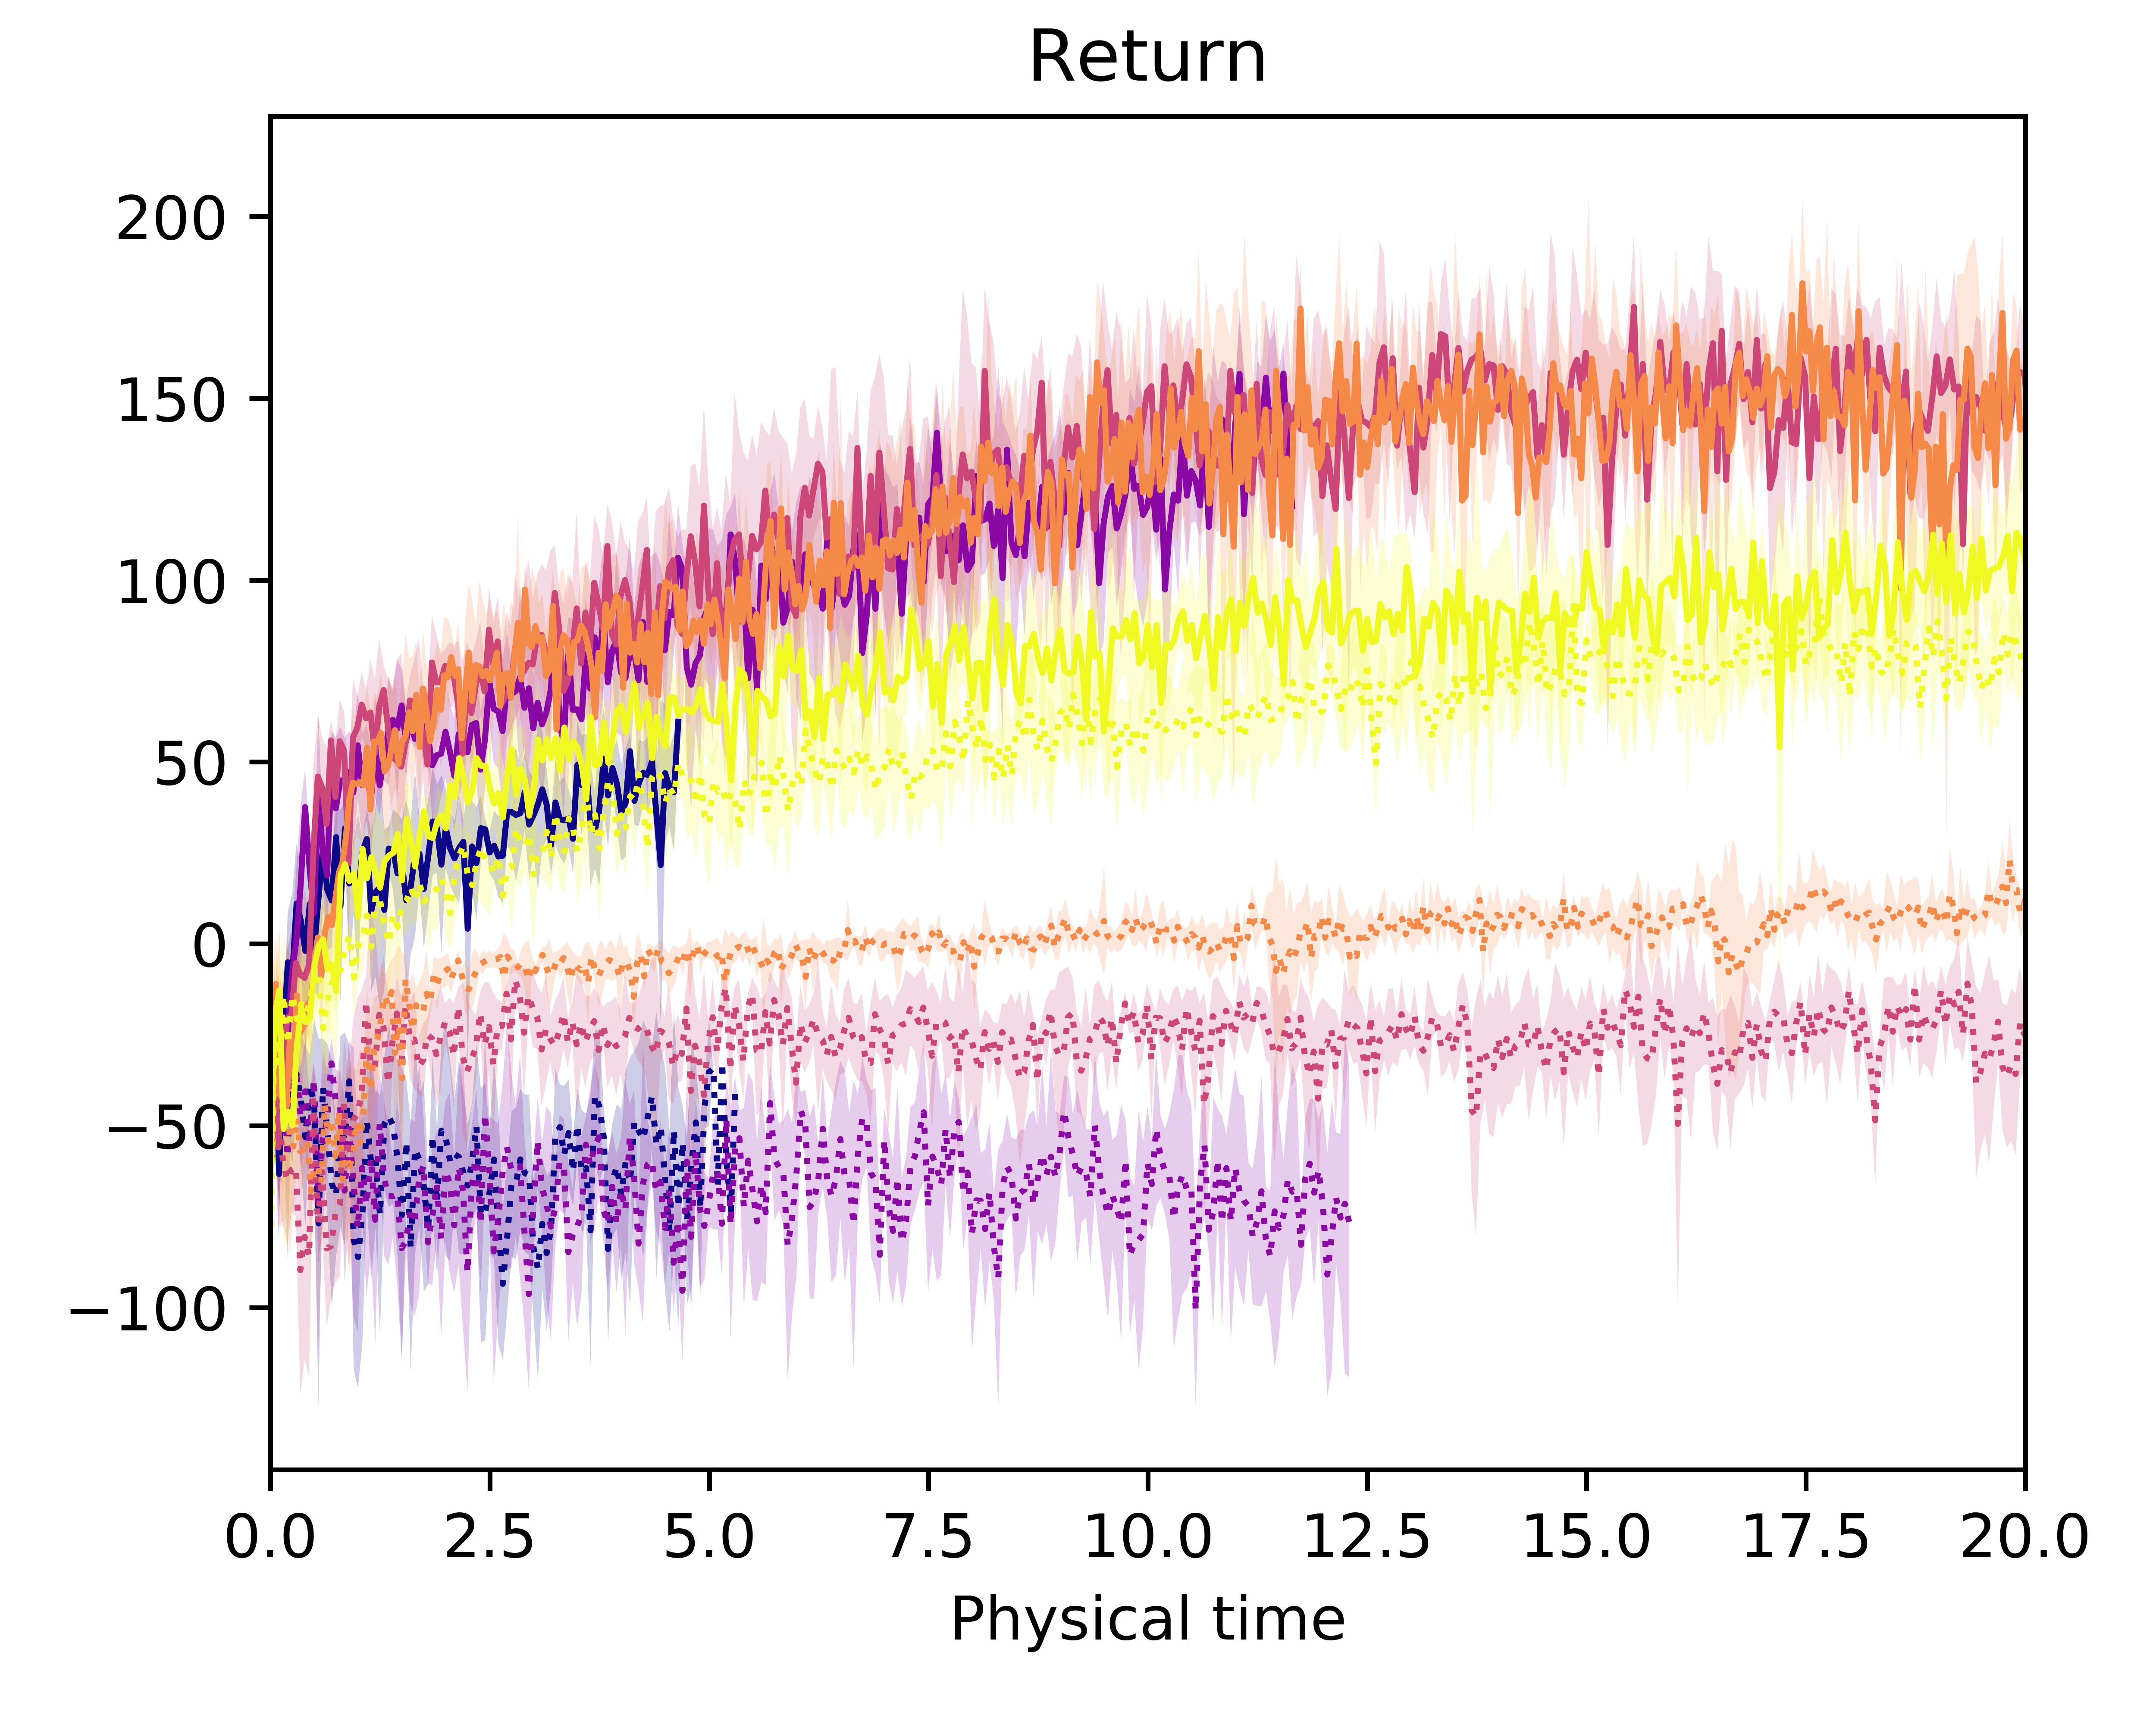
\includegraphics[width=\columnwidth]{figs_data/ant_lc.png}
%   \caption{Ant}
%   \label{fig:ant-lc}
% \end{figure}
% 
% \begin{figure}[h]
%   \centering
%   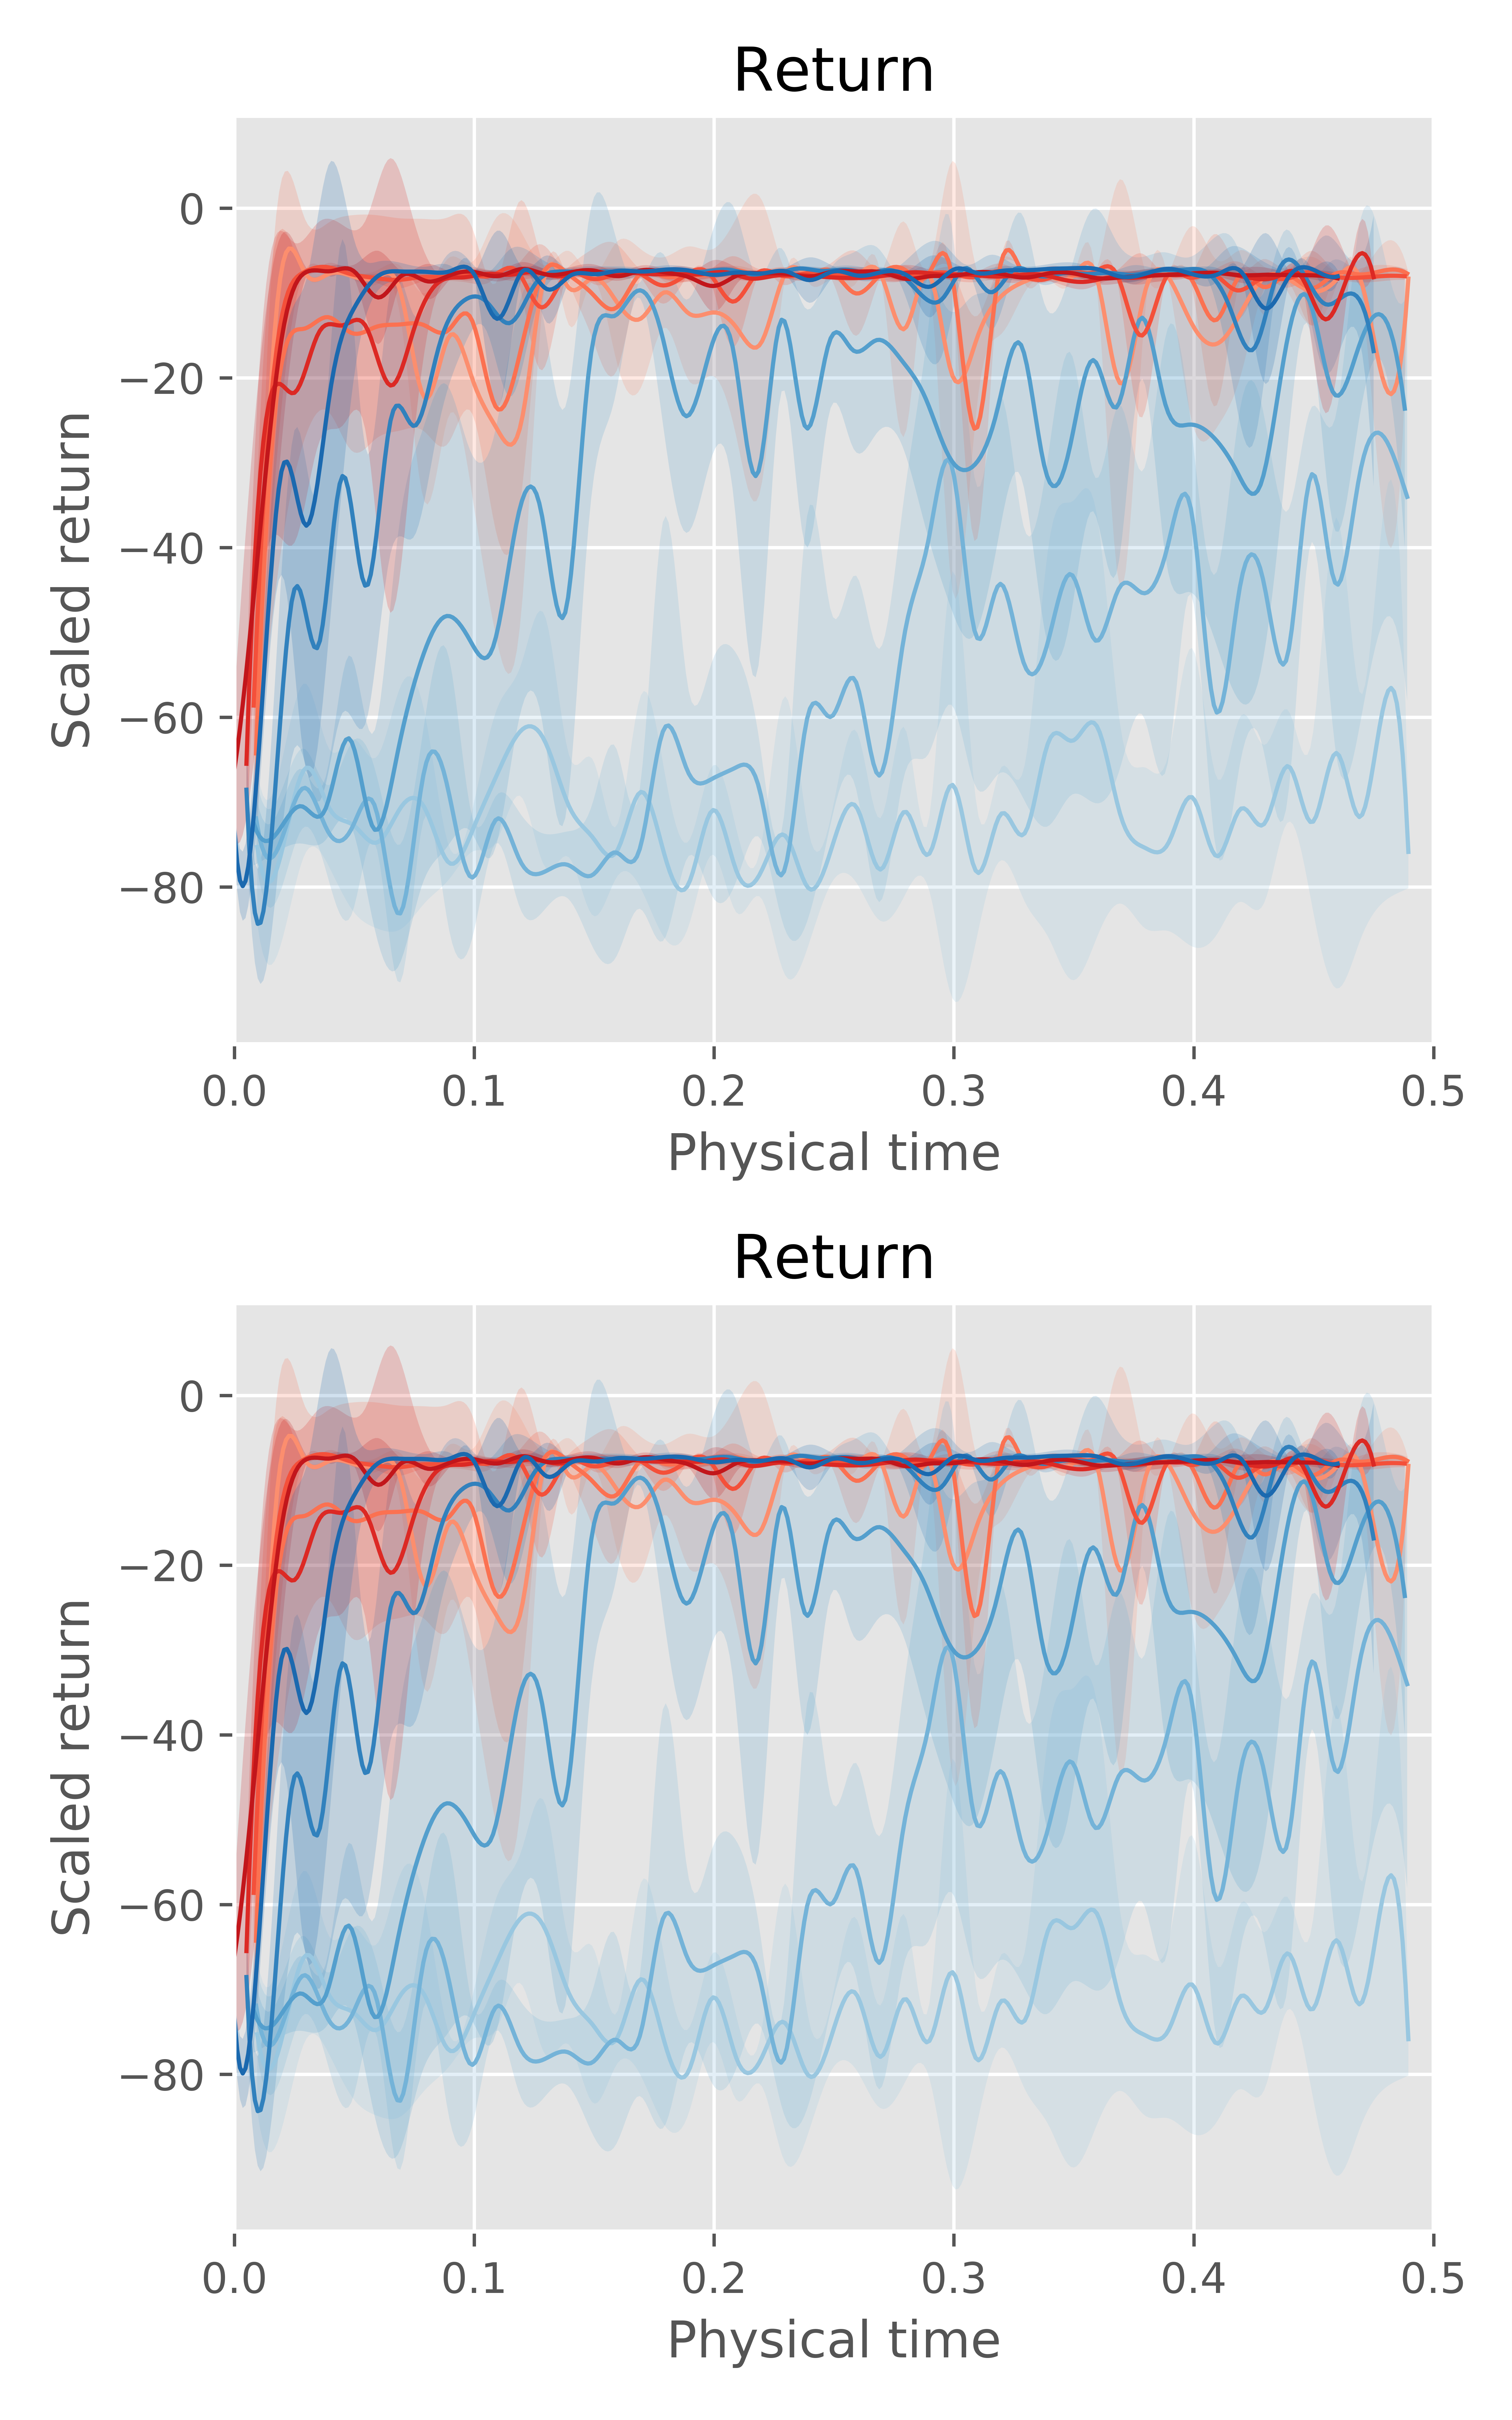
\includegraphics[width=\columnwidth]{figs_data/pendulum_lc.png}
%   \caption{Pendulum}
%   \label{fig:pendulum-lc}
% \end{figure}


%%% Local Variables:
%%% TeX-master: "icml_drau"
%%% End:
